\documentclass[tikz]{standalone}
% To convert from pdf to png use the following :
%
% C:\cygwin64\bin\convert.exe -density 600 import.pdf -resize 360x360 import.png

\usepackage{listings}

\usetikzlibrary{positioning}
\usetikzlibrary{calc}
\usetikzlibrary{backgrounds}

\begin{document}
%
% Import :
%
% This traps the import at __import__ to perform a quick swap.
%
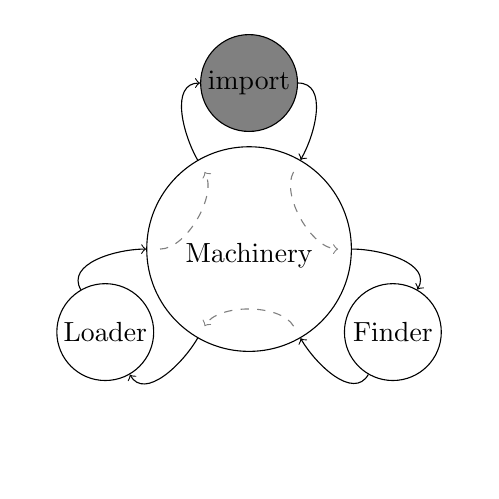
\begin{tikzpicture}[]
% Bounding Box
\path[use as bounding box] (-8em,-8em) rectangle (8em,8em);
% \draw circle (8em);
% Center
\coordinate (ctr) {}; % Used as an anchor for later nodes
% Import Mechanism
\node (imp) at ($(ctr) + ( 90:6em)$) [circle, draw, inner sep = 0.1 em, minimum size=3.5 em, fill=gray] {\lstinline|import|};
\node (fdr) at ($(ctr) + (-30:6em)$) [circle, draw, inner sep = 0.1 em, minimum size=3.5 em,          ] {\lstinline|Finder|};
\node (ldr) at ($(ctr) + (210:6em)$) [circle, draw, inner sep = 0.1 em, minimum size=3.5 em,          ] {\lstinline|Loader|};
\node (int) at (ctr)                 [circle, draw, inner sep = 1.0 em,                   align=center] {\\ Machinery};
% Internal Structure
\draw[->, shorten >=0.5em, shorten <=0.5em, gray, dashed]  (int.60) to [out = 240, in = 180]   (int.0);
\draw[->, shorten >=0.5em, shorten <=0.5em, gray, dashed] (int.180) to [out =   0, in = -60] (int.120);
\draw[->, shorten >=0.5em, shorten <=0.5em, gray, dashed] (int.300) to [out = 120, in =  60] (int.240);
% External Structure   
\draw[->] (int) to [in =  60, out =   0] (fdr);
\draw[->] (fdr) to [in = 300, out = 240] (int);
\draw[->] (int) to [in = 180, out = 120] (imp);
\draw[->] (imp) to [in =  60, out =   0] (int);
\draw[->] (int) to [in = 300, out = 240] (ldr);
\draw[->] (ldr) to [in = 180, out = 120] (int);
\end{tikzpicture}
\end{document}